\documentclass{article}
\usepackage[spanish]{babel}
\usepackage[utf8]{inputenc}
\usepackage{graphicx}
\usepackage{minted}

\title{\textbf{Criptografía aplicada: Cálculo del hash SHA-256 de un bloque Bitcoin}}
\author{Javier Domínguez Gómez \\
\small{jdg@member.fsf.org} \\
\small{Fingerprint: 94AD 19F4 9005 EEB2 3384 C20F 5BDC C668 D664 8E2B}}
\date{v0.1.03 - Febrero 2019}

\begin{document}
\maketitle

\tableofcontents{}

\section{Introducción}
    Este documento describe en detalle las partes de la cabecera de un bloque cualquiera en la cadena de bloques de Bitcoin, así como las operaciones lógico-matemáticas que se emplean con el fin de generar el \textit{hash} adecuado tras aplicar la función SHA-256.
    
    \vspace{3mm}
    En primer lugar se ha de tener en cuenta que cada bloque de la cadena de bloques de Bitcoin
    \begin{figure}[H]
    \centering
        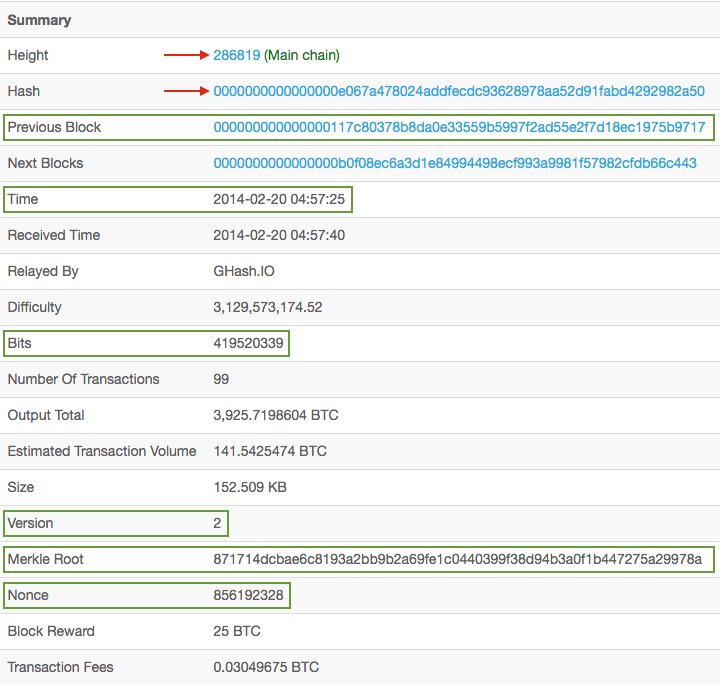
\includegraphics[scale=0.47]{img/Bitcoin_block_SHA_256_Block_Data}
        \caption{Datos empleados para la obtención del \textit{hash} del bloque $286819$.}
    \end{figure}
    
    \vspace{3mm}
    En la siguiente figura se detalla el contenido de los primeros 16 registros de la variable $W_{t}$ en cada una de las tres veces que se ejecutan las 64 iteraciones de la función SHA-256 para obtener el \textit{digest} en cada caso.
    \begin{figure}[H]
    \centering
        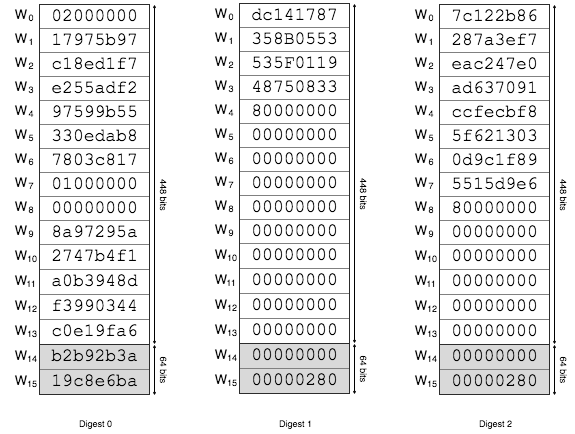
\includegraphics[scale=0.59]{img/Bitcoin_block_SHA_256_W0_W15_x3}
        \caption{Los primeros 16 registros de la variable $W_{t}$ en los tres casos en los que se ha de ejecutar la función SHA-256.}
    \end{figure}
    
\end{document}
